% !TeX spellcheck = en_US

\subsection{First-Order System}
Subsequently, we reformulate Eq. \eqref{eq:rlc_second_order_1} to yield a first-order system in the common state space formulation
\begin{align*}
	\dot{x}(t) =&~ A~ x(t) + B~\mu(t)\\
	y(t) =&~ C^\top~x(t)
\end{align*}
with states $x:[0,T]\rightarrow \mathbb{R}^{2N}$, control input signal $\mu:[0,T]\rightarrow \mathbb{R}$, output signal $y:[0,T]\rightarrow \mathbb{R}$, system matrix $A \in \mathbb{R}^{2N\times2N}$, and vectors $B, C \in \mathbb{R}^{2N}$. Hence, we firstly find
\begin{equation}
	\ddot{z}(t) + M^{-1}~D ~ \dot{z}(t) + M^{-1}~S ~ z(t) = M^{-1}~G ~ \mu(t)	 \label{eq:rlc_second_order_2}
\end{equation}
where we specify the matrices 
\begin{equation}
	A_{I} = -M^{-1}~S \quad \text{and} \quad A_{II} := -M^{-1}~D	\label{eq:first_order_submatrices}
\end{equation}
and vector $\tilde{G}:= M^{-1}~G$, and we note secondly 
\begin{equation*}
	\ddot{z}(t) = A_{I} ~ z(t)  + A_{II} ~ \dot{z}(t) + \tilde{G} ~ z(t) \text{.}
\end{equation*}
We introduce the new states $x(t) = \left[x_{1}(t),x_{2}(t)\right]$ with $x_{1}(t) = z(t)$, $x_{2}(t) = \partial_{t} z(t)$, and we define the voltage at the last shunt as our output signal 
\begin{equation}
	y(t) := z_{N}(t) = \left[\underbrace{0,\ldots,0}_{(N-1)\text{ zeros}},1,\overbrace{0\ldots,0}^{N \text{ zeros}}\right] 	\begin{pmatrix}
		{x}_{1} \\	
		{x}_{2}
	\end{pmatrix} = C^{\top} x(t) \text{.} 
\end{equation}
So, we formulate the state space as 
\begin{subequations}
\begin{align}
	\begin{pmatrix}
		\dot{x}_{1} \\	
		\dot{x}_{2}
	\end{pmatrix}
	=&~
	\underbrace{
		\begin{pmatrix}
			0 & I \\
			A_{\mathrm{I}} & A_{\mathrm{II}}
		\end{pmatrix}
	}_{=: A}
	\begin{pmatrix}
		{x}_{1} \\	
		{x}_{2}
	\end{pmatrix}
	+
	\underbrace{
		\begin{pmatrix}
			0  \\
			\tilde{G}
		\end{pmatrix}
	}_{=: B}
	\mu(t) \label{eq:state_space1}
	\text{,} \\
	y(t) =&~ C^\top ~ x(t) \text{.} \label{eq:state_space2}
\end{align}
\end{subequations}
In Eq. \eqref{eq:state_space1}, in matrix $A$ we assume a zero sub-matrix $0 = 0_{N\times N}$ and in vector $B$ we mean a row vector $0 = 0_{N}$.
If matrix $M$ in Eq. (\ref{eq:rlc_second_order_1},\ref{eq:rlc_second_order_2}) is not well conditioned, i.e. $M$ has a large condition number $\kappa = \frac{\max_{i} |\lambda_{i}|}{\min_{i} |\lambda_{i}|} \gg 1$ with eigenvalues $\lambda_{i}$ and $i \in \{1,\ldots,2N\}$, then a numerical computation of sub-matrices $A_{\mathrm{I}}$ and $A_{\mathrm{II}}$ as in Eq. \eqref{eq:first_order_submatrices} might be prone to numerical errors. Hence, we find a inverse matrix $M^{-1}$ and the concluding multiplications, Eq. \eqref{eq:first_order_submatrices}, in a closed form. We have matrix $M$ either in a triangular shape, see Eq. \eqref{eq:triangular_matrix}, or as a finite difference stencil, see Eq. \eqref{eq:finite_diff_stencil}. Thus, we have three types of matrix multiplications as sketched in  Fig. \ref{fig:matrix_multiplication} and we derive them subsequently.



\begin{marginfigure}
	\centering
	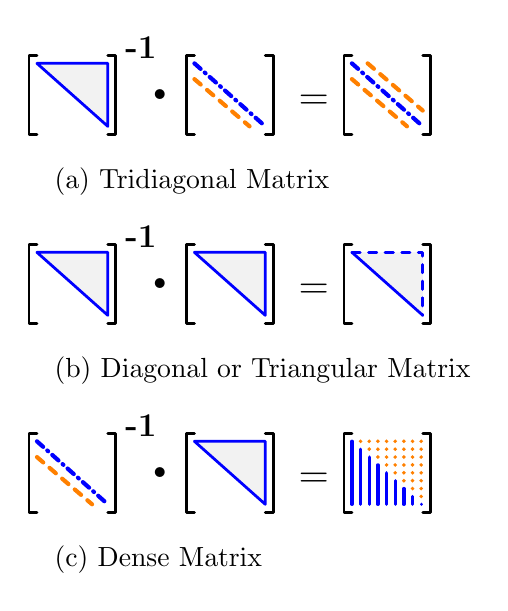
\begin{tikzpicture}[scale=1,line cap=round,line join=round,x=1.0cm,y=1.0cm]	
		\def\dx{2};
		\def\dy{-2.4};
		
		\foreach \i in {1, 2, 3}
		{
			\draw[line width=1.0] (0.1+\i*\dx,0+\dy) -- (0+\i*\dx,0+\dy) -- (0+\i*\dx,1+\dy) -- (0.1+\i*\dx,1+\dy);
			\draw[line width=1.0] (1.0+\i*\dx,0+\dy) -- (1.1+\i*\dx,0+\dy) -- (1.1+\i*\dx,1+\dy) -- (1.0+\i*\dx,1+\dy);
		}
		
		
		\draw[line width=1, color=blue, fill=gray!10] (0.1+\dx, 0.9+\dy) -- (1.0+\dx, 0.9+\dy) -- (1.0+\dx, 0.1+\dy) -- cycle;
		
		\draw[dash dot,line width=1.5, color=blue] (0.1+2*\dx,0.9+\dy) -- (1.+2*\dx,0.1+\dy);
		\draw[dashed,line width=1.5, color=orange] (0.1+2*\dx,0.7+\dy) -- (0.8+2*\dx,0.1+\dy);
		
		\draw[dash dot,line width=1.5, color=blue] (0.1+3*\dx,0.9+\dy) -- (1.+3*\dx,0.1+\dy);
		\draw[dashed,line width=1.5, color=orange] (0.1+3*\dx,0.7+\dy) -- (0.8+3*\dx,0.1+\dy);
		\draw[dashed,line width=1.5, color=orange] (0.3+3*\dx,0.9+\dy) -- (1.0+3*\dx,0.3+\dy);
		
		\node[right] at (1.1+\dx, 1.1+\dy) {\large \textbf{-1}};		
		\node[right] at (1.4+\dx, 0.5+\dy) {\Huge \textbf{.} };		
		\node[right] at (1.3+2*\dx, 0.4+\dy) {\Large = };
		
		\node[right] at (0.2+\dx, -0.6+\dy) {(a) Tridiagonal Matrix};		
		
		%%%% 2. Multiplication
		\foreach \i in {1, 2, 3}
		{
			\draw[line width=1.0] (0.1+\i*\dx,0+2*\dy) -- (0+\i*\dx,0+2*\dy) -- (0+\i*\dx,1+2*\dy) -- (0.1+\i*\dx,1+2*\dy);
			\draw[line width=1.0] (1.0+\i*\dx,0+2*\dy) -- (1.1+\i*\dx,0+2*\dy) -- (1.1+\i*\dx,1+2*\dy) -- (1.0+\i*\dx,1+2*\dy);
		}
		\draw[line width=1, color=blue, fill=gray!10] (0.1+\dx, 0.9+2*\dy) -- (1.0+\dx, 0.9+2*\dy) -- (1.0+\dx, 0.1+2*\dy) -- cycle;
		
		\draw[line width=1, color=blue, fill=gray!10] (0.1+2*\dx, 0.9+2*\dy) -- (1.0+2*\dx, 0.9+2*\dy) -- (1.0+2*\dx, 0.1+2*\dy) -- cycle;
		
		\fill[fill=gray!10] (0.1+3*\dx, 0.9+2*\dy) -- (1.0+3*\dx, 0.9+2*\dy) -- (1.0+3*\dx, 0.1+2*\dy) -- cycle;
		\draw[dashed, line width=1, color=blue] (0.1+3*\dx, 0.9+2*\dy) -- (1.0+3*\dx, 0.9+2*\dy) -- (1.0+3*\dx, 0.1+2*\dy);
		\draw[solid, line width=1, color=blue] (0.1+3*\dx, 0.9+2*\dy) -- (1.0+3*\dx, 0.1+2*\dy);
		
		\node[right] at (1.1+\dx, 1.1+2*\dy) {\large \textbf{-1}};		
		\node[right] at (1.4+\dx, 0.5+2*\dy) {\Huge \textbf{.} };		
		\node[right] at (1.3+2*\dx, 0.4+2*\dy) {\Large = };
		
		\node[right] at (0.2+\dx, -0.6+2*\dy) {(b) Diagonal or Triangular Matrix};		
		
		
		%%%% 3. Multiplication
		\foreach \i in {1, 2, 3}
		{
			\draw[line width=1.0] (0.1+\i*\dx,0+3*\dy) -- (0+\i*\dx,0+3*\dy) -- (0+\i*\dx,1+3*\dy) -- (0.1+\i*\dx,1+3*\dy);
			\draw[line width=1.0] (1.0+\i*\dx,0+3*\dy) -- (1.1+\i*\dx,0+3*\dy) -- (1.1+\i*\dx,1+3*\dy) -- (1.0+\i*\dx,1+3*\dy);
		}
		
		
		\draw[dash dot,line width=1.5, color=blue] (0.1+\dx,0.9+3*\dy) -- (1.0+\dx,0.1+3*\dy);
		\draw[dashed,line width=1.5, color=orange] (0.1+\dx,0.7+3*\dy) -- (0.8+\dx,0.1+3*\dy);
		
		\draw[line width=1, color=blue, fill=gray!10] (0.1+2*\dx, 0.9+3*\dy) -- (1.0+2*\dx, 0.9+3*\dy) -- (1.0+2*\dx, 0.1+3*\dy) -- cycle;
		
		
		\draw[line width=1.2, color=blue] (0.1+3*\dx, 0.9+3*\dy) -- (0.1+3*\dx, 0.1+3*\dy);
		\foreach \i in {1, ..., 8}
		{
			\draw[line width=1.2, color=blue] (0.1+\i*0.11+3*\dx, 0.9-\i*0.1+3*\dy) -- (0.1+\i*0.11+3*\dx, 0.1+3*\dy);
			\foreach \j in {1, ..., \i}
			{
				\fill [line width=1.0, color=orange] (0.1+\i*0.11 +3*\dx, 1.0 -0.1*\j +3*\dy) circle [radius = 0.025];	
			}
		}
		
		
		
		\node[right] at (1.1+\dx, 1.1+3*\dy) {\large \textbf{-1}};		
		\node[right] at (1.4+\dx, 0.5+3*\dy) {\Huge \textbf{.} };		
		\node[right] at (1.3+2*\dx, 0.4+3*\dy) {\Large = };
		
		\node[right] at (0.2+\dx, -0.6+3*\dy) {(c) Dense Matrix};	
		
		
	\end{tikzpicture}
	\caption{Matrix multiplications.}
	\label{fig:matrix_multiplication}
\end{marginfigure}

\subsection*{Inverse Triangular Matrix}
To compute sub-matrices $A_{\mathrm{I}}$ and $A_{\mathrm{II}}$ for circuit types (a) and (b), we have matrix $\mathbf{M}$ in a triangular form $\mathbf{T}_{a,b}$, see Eq. \eqref{eq:triangular_matrix}. We find the inverse of $\mathbf{T}_{a,b}$ as the upper finite difference stencil shape 
\begin{align*}
	\mathbf{T}_{a,b}^{-1} = 
	\begin{pmatrix}
		\frac{1}{a_{1} ~ b_{1}} & \frac{-1}{a_{2} ~ b_{1}} & 0  						& \cdots & 0 \\[1ex]
		0 						 &   \frac{1}{a_{2} ~ b_{2}} & \frac{-1}{a_{3} ~ b_{2}} &  & \vdots \\
		\vdots 				 		 &  \ddots 					 & \ddots 					 & \ddots & 0	 \\
		&  & 0 & \frac{1}{a_{N-1} ~ b_{N-1}} & \frac{-1}{a_{N} ~ b_{N-1}} \\[1ex]
		0  & \cdots 	& &  			0			   & \frac{1}{a_{N} ~ b_{N}} 
	\end{pmatrix} \text{.}
\end{align*}

Here, we distinguish two scenarios: a multiplication of $\mathbf{T}^{-1}$ with a finite difference stencil $\mathbf{F}$, see Eq. \eqref{eq:finite_diff_stencil}, and with triangular matrix $\mathbf{T}$. In the first case, we define the resulting matrix as
\begin{equation}
	\mathbf{L}_{\alpha,\beta} := -\mathbf{T}_{a,b}^{-1} ~\cdot~ \mathbf{F}
\end{equation}
and we see that it is a tridiagonal matrix\sidenote{\color{red} We also call this Laplacian matrix (side note with link to wiki)} as
\begin{equation}
	\mathbf{L}_{\alpha,\beta} =
	\begin{pmatrix}
		\gamma_{1} & \beta_{1} \\
		\alpha_{2} & \gamma_{2} & \beta_{2} \\
		& \ddots & \ddots & \ddots \\
		& & \alpha_{N-1} & \gamma_{N-1} & \beta_{N-1} \\
		& & & \alpha_{N} & -\alpha_{N}
	\end{pmatrix}
\end{equation}
with sub-diagonal entries
\begin{equation}
	\alpha_{n} = \frac{1}{a_{n}~ b_{n}} ~ \text{,} \quad 
	\beta_{n} =  \frac{1}{a_{n+1}~ b_{n}} \\
\end{equation}
and diagonal elements
\begin{equation*}
	\gamma_{n} = -\left[\alpha_{n}+\beta_{n}\right]
\end{equation*}
for $n\in\{1,\ldots,N\}$. Matrix shape $\mathbf{L}_{\alpha,\beta}$ is portrayed in Fig. \ref{fig:matrix_multiplication} (a).

In the second case, we have the second upper triangular matrix as $\mathbf{T}_{\tilde{a},\tilde{b}}$ with coefficients $\tilde{a}_{n}$ and $\tilde{b}_{n}$ for $n\in\{1,\ldots,N\}$. We define the product as 
\begin{equation}
	\mathbf{P}_{\alpha,\beta} := - \mathbf{T}_{a,b}^{-1} ~ \cdot ~ \mathbf{T}_{\tilde{a},\tilde{b}}
\end{equation}
which has a triangular form again, see Fig. \ref{fig:matrix_multiplication} (b), as
\begin{equation}
	P_{\alpha,\beta} = 
	\begin{pmatrix}
		\alpha_{1} & \beta_{1,2} &  \beta_{1,3} & \ldots &   \beta_{1,N} \\
		& \alpha_{2} & \beta_{2,3} &  \ldots &  \beta_{2,N} \\
		& & \ddots & \vdots \\
		& & & \alpha_{N-1} & \beta_{N-1,N} \\
		& & & & \alpha_{N}
	\end{pmatrix}
\end{equation}
with entries
\begin{equation}
	\alpha_{n} = \frac{\tilde{a}_{n}}{a_{n}} \quad \text{and} \quad \beta_{n,k} = \left[\frac{\tilde{a}_{n}}{a_{n}} - \frac{\tilde{a}_{n+1}}{a_{n+1}} \right] \frac{\tilde{b}_{k}}{b_{n}} \text{.}
\end{equation} 
In Table \ref{table:triangular_matrix_values}, we see that the coefficients $b_{n}$ are equal for both triangular matrices and so we have $\tilde{b}_{k} \equiv b_{k}$ for $k \in \{1,\ldots,N\}$. The coefficients $a_{n}$ and $\tilde{a}_{n}$ differ in general, but if they are scaled\sidenote{\color{red} (Side Note: this is in particular the case if all values of the related electrical elements are equals. Simple RLC example...)} as  $\tilde{a} = \epsilon a_{n}$ for all $n \in \{1,\ldots,N\}$ with $\epsilon \in \mathbb{R}$, then we yield a pure diagonal matrix
\begin{equation*}
	\mathbf{P}_{\alpha,\beta} = \epsilon~\mathbf{I} \text{.}
\end{equation*}
with identity matrix $\mathbf{I} =\operatorname{diag}(1,\ldots,1)$.

The input signal $\mu$ is scaled by vector $B = [0, \tilde{G}]^\top$ and we find $\tilde{G}$ as 
\begin{equation}
	\tilde{G} ~=~ \mathbf{T}_{a,b}^{-1} ~ G = \mathbf{T}_{a,b}^{-1} ~ 
	\begin{pmatrix}
		1 \\
		0 \\
		\vdots \\
		0
	\end{pmatrix} ~=~
	\begin{pmatrix}
		\frac{1}{a_{1} ~ b_{1}} \\
		0 \\
		\vdots \\
		0
	\end{pmatrix}
\end{equation}
and further, we yield
\begin{equation*}
	B = 
	\begin{pmatrix}
		0 \\
		\vdots \\
		0 \\
		\frac{1}{a_{1} ~ b_{1}} \\
		0 \\
		\vdots \\
		0
	\end{pmatrix}
	\begin{matrix}
		\\
		\\
		\\
		\leftarrow (N+1)\text{-th position}\\
		\\
		\\
		~
	\end{matrix}
	\textbf{.}
\end{equation*}

\subsection*{Inverse Finite Difference Stencil}

In case of ladder type (c), we need to evaluate another matrix multiplication. Here, we invert the finite difference stencil $\tilde{F}$ and we obtain a lower triangular matrix
\begin{equation*}
	\mathbf{F}^{-1} =
	\begin{pmatrix}
		1 & 0  &  0\\
		\vdots 	& \ddots &  0 \\
		1 &	\cdots	 &     1 
	\end{pmatrix} \text{.}
\end{equation*}
We multiply this lower triangular matrix with $\mathbf{T}_{a,b}$ as in Eq. \eqref{eq:triangular_matrix} and we define the result as 
\begin{equation}
	\mathbf{Q} := - \mathbf{F}^{-1} ~\cdot~ \mathbf{T}_{a,b}
\end{equation}
where $\mathbf{Q} = [q_{n,k}]$ with entries
\begin{equation}
	q_{n,k} = b_{k} \sum_{i=1}^{\min\{n,k\}} a_{i}
\end{equation}
for $n,k \in \{1,\ldots,N\}$. The resulting matrix shape is illustrated in Fig. \ref{fig:matrix_multiplication} (c). If all values of $b_{k}$ are equal as
\begin{equation}
	b_{1}=\ldots=b_{N}~=:~\tilde{b}	\text{,}
\end{equation}
\begin{marginfigure}
	\centering
	\begin{tikzpicture}[scale=1,line cap=round,line join=round,x=1.0cm,y=1.0cm]	
		\node at (-1,1) {\huge $\mathbf{Q}=$ };
		\draw[line width=1] (0.3, -0.05) -- (0, -0.05) -- (0, 2.05) -- (0.3, 2.05);
		\draw[line width=1] (1.9, -0.05) -- (2.2, -0.05) -- (2.2, 2.05) -- (1.9, 2.05);
		
		\draw[line width=2,color=wong1] (0.2,0.1) -- (0.2,1.9) -- (2.0,1.9);
		
		
		\def\dx{0.2}
		\draw[line width=2,color=wong2] (0.2+\dx,0.1) -- (0.2+\dx,1.9-\dx) -- (2.0,1.9 -\dx);
		\draw[line width=2,color=wong3] (0.2+2*\dx,0.1) -- (0.2+2*\dx,1.9-2*\dx) -- (2.0,1.9 -2*\dx);
		\draw[line width=2,color=wong4] (0.2+3*\dx,0.1) -- (0.2+3*\dx,1.9-3*\dx) -- (2.0,1.9 -3*\dx);	
		
		
		\draw[line width=2,color=wong5] (0.2+7*\dx,0.1) -- (0.2+7*\dx,1.9-7*\dx) -- (2.0,1.9 -7*\dx);
		\draw[line width=2,color=wong6] (0.2+8*\dx,0.1) -- (0.2+8*\dx,1.9-8*\dx) -- (2.0,1.9 -8*\dx);
		%	\draw[line width=2,color=blue] (0.2+9*\dx,0.1) -- (0.2+9*\dx,1.9-9*\dx) -- (2.0,1.9 -9*\dx);
		\fill [line width=1.0, color=juliapurple] (0.2+8.8*\dx,1.9-8.8*\dx) circle [radius = 0.06];	
		
		\fill [line width=1.0, color=blue] (0.2+4.3*\dx,1.9-4.3*\dx) circle [radius = 0.05];	
		\fill [line width=1.0, color=blue] (0.2+5*\dx,1.9-5*\dx) circle [radius = 0.05];	
		\fill [line width=1.0, color=blue] (0.2+5.7*\dx,1.9-5.7*\dx) circle [radius = 0.05];	
	\end{tikzpicture}
	\caption{Illustraion of symmetric dense matrix $Q$ where common rows and columns have equal entries.}
	\label{fig:dense_matrix}
\end{marginfigure}
then this matrix multiplication results in a symmetric shape
\begin{equation*}
	\mathbf{Q} =~ 
	\def\aa{\color{red}\tilde{q}_{2}}
	\def\ab{\color{red}\tilde{q}_{N-1}}
	\begin{pmatrix}
		\tilde{q}_{1} & \tilde{q}_{1} & \tilde{q}_{1} & \ldots & \tilde{q}_{1} & \tilde{q}_{1} \\
		\tilde{q}_{1} & \aa & \aa & \ldots & \aa & \aa \\
		& \aa & \tilde{q}_{3} & \ldots & \tilde{q}_{3} & \tilde{q}_{3} \\
		\vdots     & \vdots & \vdots & \ddots \\
		\tilde{q}_{1}& \aa & \tilde{q}_{3} & & \ab & \ab \\
		\tilde{q}_{1} & \aa & \tilde{q}_{3} & & \ab & \tilde{q}_{N}
	\end{pmatrix} \\
\end{equation*}
with $\tilde{q}_{n} = \tilde{b} ~ \sum\limits_{i=1}^{n} a_{i}$, see Fig. \ref{fig:dense_matrix} for illustration.

We note the scaling vector $B$ of input signal $\mu$ in this case as
\begin{equation*}
	B = 
	\begin{pmatrix}
		0 \\
		\vdots \\
		0 \\
		1 \\
		1 \\
		\vdots \\
		1
	\end{pmatrix}
	\begin{matrix}
		\\
		\\
		\\
		\leftarrow (N+1)\text{-th position}\\
		\\
		\\
		~
	\end{matrix}
\end{equation*}
because we have here $\tilde{G} = \mathbf{F}^{-1}~G = \left[1,\ldots,1\right]^\top$.